%% Technical report, team brasileirao, More than a Hack 2027 (Phase 1: ball possession).
%% Compiles with pdflatex on Overleaf (IEEEtran is part of TeX Live).
%% Every number in this document comes from external data (degraded IDSSE matches).
%% No value derived from the provided match appears here, and no public-window score.

\documentclass[journal]{IEEEtran}

\usepackage[utf8]{inputenc}
\usepackage[T1]{fontenc}
\usepackage{amsmath}
\usepackage{booktabs}
\usepackage{array}
\usepackage{tikz}
\usetikzlibrary{positioning,arrows.meta}
\usepackage{pgfplots}
\pgfplotsset{compat=1.17}
\usepackage[hidelinks]{hyperref}

\newcommand{\spf}{\textsc{spellF1}}
\newcommand{\mf}{\textsc{macroF1}}
\newcommand{\cfg}[1]{\texttt{#1}}

\begin{document}

\title{Frame-level Ball Possession with a Hidden Markov Model over Calibrated, Stacked Evidence}

\author{Team \texttt{brasileirao}: Ahmed~Amer~Hachem, Antônio~Escobar~Torres, Bernardo~Silva~Andrade, Fernando~Horita~Siratuti and Hugo~Henrique~Marques%
\thanks{More than a Hack 2027, Phase 1 (ball possession). FC Barcelona (home, \texttt{H}) vs Athletic Club (away, \texttt{A}), LaLiga 2024--25, matchday 2.}%
\thanks{Code: \url{https://github.com/AntonioEscobarTorres/more-than-a-hack-2027-brasileirao}, tag \texttt{submission-v1.1}.}}

\markboth{More than a Hack 2027 --- Technical report, team brasileirao, November~2026}%
{Team brasileirao: Frame-level ball possession with an HMM over calibrated evidence}

\maketitle

\begin{abstract}
We label every frame of the tactical video as home possession, away possession or dead ball with a three-state hidden Markov model (HMM) decoded offline with Viterbi, one half at a time. Its inputs are per-frame log-likelihood ratios that read zero when there is no evidence, so a frame without a ball keeps the previous state, which is the challenge rule for a loose ball. The evidences are gradient-boosted trees over features of the automatic tracking: who controls the ball, whether the ball is dead, and a hazard of a change of possession. Second-stage models then read these evidences in past and future windows, and the hazard also modulates the exits of the decoder. No label of the provided match was used. Every model, weight and decoder parameter was fitted and chosen on seven public matches of the IDSSE dataset, degraded to look like automatic tracking, with one match left out at a time and a fixed acceptance rule. Under that protocol the final system reaches a mean \spf{} of 0.567 (0.541--0.598 across five degradation modes), against 0.173 for a rule-based baseline. We also report the variants that the protocol rejected, and the limits of this estimate.
\end{abstract}

\begin{IEEEkeywords}
Ball possession, tracking data, hidden Markov model, gradient boosting, stacking, domain shift, football.
\end{IEEEkeywords}

\section{Approach and why}
\label{sec:approach}

\subsection{The problem as we read it}
The ranking metric, \spf{}~\cite{mtah2027}, matches whole possessions, not frames. A label that flickers creates many false possessions, and a boundary that arrives late lowers the overlap of two possessions at once. A per-frame classifier can look good on \mf{} and still fail on \spf{}. Two other facts shaped the design: the tactical ball is missing in about 41\,\% of the graded frames (DATA.md), and no label of the provided match may be used to train or choose anything. Every parameter therefore had to come from other matches, and the method had to survive the change from that data to the provided tracking.

\subsection{Pipeline}
Fig.~\ref{fig:pipeline} shows the pipeline. One command runs all of it.

\begin{figure}[t]
\centering
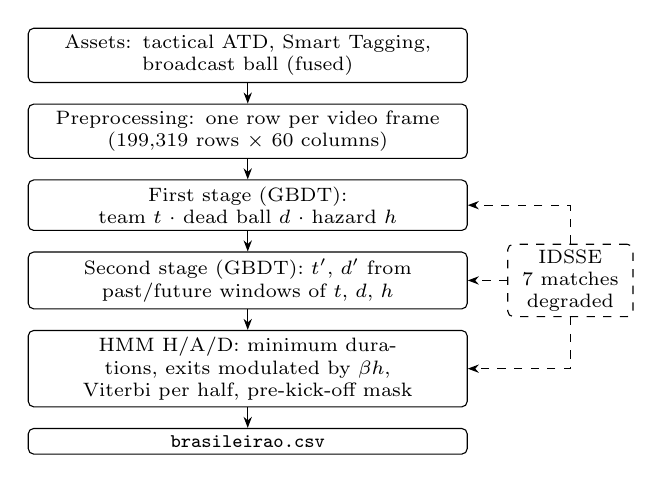
\begin{tikzpicture}[
  font=\scriptsize,
  box/.style={draw, rounded corners=2pt, align=center, text width=5.4cm, inner sep=2.5pt},
  side/.style={draw, dashed, rounded corners=2pt, align=center, text width=1.45cm, inner sep=2pt},
  arr/.style={-{Stealth[length=4pt]}},
  node distance=2.6mm]
\node[box] (raw) {Assets: tactical ATD, Smart Tagging,\\broadcast ball (fused)};
\node[box, below=of raw] (pre) {Preprocessing: one row per video frame\\(199{,}319 rows $\times$ 60 columns)};
\node[box, below=of pre] (s1) {First stage (GBDT):\\team $t$ $\cdot$ dead ball $d$ $\cdot$ hazard $h$};
\node[box, below=of s1] (s2) {Second stage (GBDT): $t'$, $d'$ from\\past/future windows of $t$, $d$, $h$};
\node[box, below=of s2] (hmm) {HMM H/A/D: minimum durations, exits modulated by $\beta h$, Viterbi per half, pre-kick-off mask};
\node[box, below=of hmm] (csv) {\texttt{brasileirao.csv}};
\draw[arr] (raw) -- (pre);
\draw[arr] (pre) -- (s1);
\draw[arr] (s1) -- (s2);
\draw[arr] (s2) -- (hmm);
\draw[arr] (hmm) -- (csv);
\node[side, right=5mm of s2.east, anchor=west] (idsse) {IDSSE\\7 matches\\degraded};
\draw[arr, dashed] (idsse.north) |- (s1.east);
\draw[arr, dashed] (idsse.west) -- (s2.east);
\draw[arr, dashed] (idsse.south) |- (hmm.east);
\end{tikzpicture}
\caption{Pipeline. Solid arrows: inference on the provided match. Dashed: every model and decoder parameter is fitted and selected on degraded IDSSE only.}
\label{fig:pipeline}
\end{figure}

\textbf{Preprocessing.} The provided assets become one table with one row per tactical video frame and 60 columns. Positions are in metres and rotated so that the home team always attacks towards increasing $x$. A jump filter removes phantom ball detections (steps not reachable at 38\,m/s plus 1\,m of noise). Only ball gaps of up to 0.5\,s are interpolated, and kinematics come from a zero-phase Savitzky--Golay filter~\cite{savitzky1964} on observed samples only. The table also holds per-team proximity and pressure features (nearest-player distance, counts within 2, 3 and 5\,m, relative speed), team aggregates, pitch-line distances and the Smart Tagging intervals. Every inferred value is flagged, \texttt{NaN} always means ``no evidence'', and nothing is computed across halftime. All thresholds are physical priors, none tied to frames of the match.

\textbf{Evidences.} Three per-frame scores feed the decoder, each fitted on degraded IDSSE with scikit-learn's histogram gradient boosting~\cite{friedman2001,ke2017,pedregosa2011}:
\begin{itemize}
\item \emph{Team evidence} $t$ (home vs away). Its inputs are ball--player proximity, pressure and relative speed, a \emph{pass bridge} (an exponentially decaying memory of the signed control signal, which carries control across the flight of a pass), a \emph{touch} feature (the same team within 1.5\,m of the ball on at least 5 of 9 frames), collective features, and windows of 0.5--2\,s. Swapping the two teams is a signed permutation $S$ of the feature matrix, and $t=\mathrm{clip}\big((g(X)-g(SX))/2,\pm 8\big)$ is exactly antisymmetric: the model cannot learn a preference for one side. Frames without a valid ball use a small antisymmetric logistic model on collective features instead.
\item \emph{Dead-ball evidence} $d$ (dead vs live). Its inputs are the ball out of the pitch, the kind and length of a ball gap (Section~\ref{sec:rules}), the share of still players, the mean player speed, a fast ball inside the pitch and the distances to the lines, each in windows of 1--3\,s before and after the frame. The output minus the training prior log-odds is a likelihood ratio, and low-weight Smart Tagging priors are added on top.
\item \emph{Hazard} $h$: the log-odds of a change of team within the next 12 frames. Every input is symmetric under the team swap (backward vs forward smoothed control and touch signals, their products and differences, the amount of control evidence around the frame), so the hazard says \emph{whether} possession changes, never to whom.
\end{itemize}

\textbf{Second stage.} The HMM treats frames as independent given the state, so it cannot learn where the switch falls when the past says one team and the future says the other. A second GBDT per evidence (stacked generalisation~\cite{wolpert1992}) reads past and future means of the first-stage $t$ (0.25 to 8\,s), past and future maxima of $h$, and returns a new $t'$, antisymmetric by construction; the same is done for $d$ (tags added afterwards, because IDSSE has none). To avoid leakage, the fold model of held-out match $m$ is trained on matches $j\neq m$ whose first-stage inputs come from models fitted without both $m$ and $j$.

\textbf{Decoder.} A three-state HMM~\cite{rabiner1989} with emissions
\begin{equation}
\begin{split}
S_H &= \lambda_t\,(\log 2+\log\sigma(t')),\quad S_A=\lambda_t\,(\log 2+\log\sigma(-t')),\\
S_D &= \lambda_d\, d'.
\end{split}
\end{equation}
With $t'=d'=0$ all three are exactly zero and the previous state persists. Each state is a chain of substates that enforces a minimum duration (12 frames for H and A, 25 for D), followed by a geometric tail whose mean (7.6\,s, 6.8\,s and 25.2\,s) and exit split are the IDSSE statistics. In the style of an input--output HMM~\cite{bengio1995}, the hazard modulates the H/A exits at every frame: the exit to the other team is multiplied by $e^{\beta h_t}$ and the row is renormalised. Viterbi~\cite{forney1973} runs in \texttt{float64}, separately on each half. The final values are $\lambda_t=0.4$, $\lambda_d=0.4$, $\beta=1.5$.

\subsection{Why this and not something else}
\begin{itemize}
\item \emph{Global offline decoding.} It produces no flicker and, being bidirectional, no phase lag. Offline use is allowed (official issue \#15), and \spf{} punishes lag heavily (EVALUATION.md).
\item \emph{Zero means no evidence.} With likelihood-ratio evidences a missing ball contributes nothing, which implements ``loose ball stays with the last team'' without a special case.
\item \emph{Evidence models, not a per-frame classifier of the labels.} We started with interpretable priors and logistic models and moved to GBDTs only when the protocol showed a clear gain (Section~\ref{sec:validation}). The decoder and the possession rules stayed explicit.
\item \emph{Second stage.} Diagnostics on degraded IDSSE showed where the score was lost. With the team evidence replaced by the truth, the same decoder reached \spf{} 0.906; with the dead-ball evidence replaced by the truth, only 0.593. Of the 3{,}760 true boundaries, 2{,}351 are team-to-team changes in open play, and only 29\,\% of these were found within 12 frames. So the last effort went into \emph{when} the team changes.
\end{itemize}

\section{Assets used and dropped}
\label{sec:assets}

\begin{table}[t]
\caption{Assets of the provided match.}
\label{tab:assets}
\centering
\footnotesize
\begin{tabular}{@{}>{\raggedright\arraybackslash}p{1.75cm}>{\raggedright\arraybackslash}p{1.35cm}>{\raggedright\arraybackslash}p{4.55cm}@{}}
\toprule
Asset & Status & How it is used, or why not\\
\midrule
Tactical ATD & Used & Basis of everything: every feature.\\
Smart Tagging & Weak evidence & Set-piece tags add low-weight priors to $d$ only; kick-off tags only checked against the published frames.\\
Homography & Not used & Diagnostics only; reprojection error does not exist on IDSSE and is tied to match time.\\
Tactical video & Not used & Watched to debug the pipeline (e.g.\ attacking direction); never a label, correction, constant or check of the output.\\
Broadcast video & Not used & Own timeline with cuts, replays and zooms.\\
Broadcast tracking: players & Dropped & Feasibility gate NO-GO (below).\\
Broadcast tracking: ball & Used (fused) & Fills only tactical frames without a ball, where the mapping is reliable.\\
\bottomrule
\end{tabular}
\end{table}

Table~\ref{tab:assets} summarises the decisions.

\textbf{Smart Tagging as weak evidence.} The tags are automatic and have low recall for restarts, every throw-in is tagged without a team, and a set-piece interval extends past the restart. A high weight would delay the start of the next possession after every tagged restart, so dead-ball detection relies on kinematics. The phase tags describe intervals of play, not possessions, and are not model inputs.

\textbf{Homography and videos.} The tracking already carries the positions the model needs. Running our own ball detector was out of scope for the time available, and a vision model would make bit-exact CPU reproduction harder.

\textbf{Broadcast tracking.} The broadcast camera may see the ball where the tactical one does not, but it runs on its own timeline. We mapped it to the tactical timeline with no correspondence table: cross-correlation of the two ball trajectories gives coarse shifts (per half and on sliding 60\,s windows), refined on 2\,s blocks by matching each visible broadcast player with the nearest tactical player of the same team, and kept only in live segments of at least 10\,s. A gate with thresholds fixed in advance gave \textbf{NO-GO}: the mapping is accurate where it exists (player and ball agreement pass), but it covers too little of the graded frames and recovers too few of the missing tactical balls. The player track was dropped. After the gate we measured what the \emph{ball} alone adds on IDSSE, filling only tactical frames without a ball: $+0.0064\pm0.0020$ \spf{} on the candidate of that day (6 of 7 matches). We revised the decision for the ball only and put it through the same acceptance rule (Section~\ref{sec:validation}). This revision was made after the gate result was known, and we list it as such.

\section{External training data}
\label{sec:external}

\textbf{Dataset.} The only labelled data is IDSSE~\cite{bassek2025}: seven complete matches of the 2022/23 German Bundesliga and 2.~Bundesliga, with official positional data at 25\,fps and, for every frame, the ball status (alive or dead) and the team in possession. Licence: CC BY 4.0. Its use was approved by the organisers (official issue \#16). We used the Hugging Face mirror \texttt{pysport/idsse-data}~\cite{idssehf} at the pinned revision \texttt{a715a38d\ldots}, read with kloppy~\cite{kloppy}; names, sizes and SHA-256 values of the files are listed in \texttt{docs/external\_data.md}.

\textbf{Who labelled it, and how much.} The labels are part of the published dataset (DFL official data). We labelled nothing, by hand or otherwise. In total there are 1{,}002{,}644 labelled frames (about 11.1\,h): 41--52\,\% dead ball per match, the rest split between the teams. \textbf{No label comes from the provided match.}

\textbf{Degradation.} IDSSE tracking is complete and corrected; the provided ATD is automatic. Each IDSSE match is therefore degraded and then passed through the same preprocessing as the provided match:
\begin{itemize}
\item \emph{Ball:} hidden in crowds and in part of the dead balls, plus gaps drawn from a gap-length profile that are more likely during slow play, until 59.3\,\% of the frames show a ball (the figure published in DATA.md); a slow drift of the ball during dead balls; position noise; short phantom detections.
\item \emph{Players:} tracks dropped and restored until 20.5 players are tracked on average (DATA.md); position noise; short duplicated tracks.
\end{itemize}
The parameters of the degradation were adjusted until label-free statistics of degraded IDSSE (player and ball speed, stationary ball, long gaps, ball visibility by player speed, tracked players) matched those of the provided tracking within $\pm$20\,\%; the divergences that remain are listed in Section~\ref{sec:limits}. As an independent check, the organisers' starter \texttt{baseline\_smooth50} scores \spf{} 0.254 on degraded IDSSE, against the 0.243 the organisers published for the full provided match. All random draws use fixed seeds.

\textbf{Stress modes.} Because the degradation is only an approximation, every step is also evaluated on four other versions: \texttt{harder} and \texttt{easier} (ball visible on 50\,\% and 68\,\% of frames, more and fewer phantoms, 20.0 and 21.3 tracked players), and \texttt{hidelo} and \texttt{hidehi} (ball hidden in 25\,\% and 75\,\% of dead balls instead of 50\,\%). A sixth version, \texttt{fused}, matches the ball visibility of the fused master.

\section{Possession rules implemented}
\label{sec:rules}

\textbf{Loose ball: persistence.} A frame with no evidence (no ball, or players too far to decide) has $t'=0$ and adds nothing, so the decoder keeps the last team. Possession changes only when the evidence for the other team outweighs the cost of a transition and the minimum duration. A pass is bridged by the control memory in $t$, so the passing team keeps possession during the flight of the ball.

\textbf{Challenges and duels.} When both teams have a player within 2\,m of the ball the contact is marked as \emph{contested}, an input of the team evidence (in the prior model its weight is halved). A deflection or a short touch without control does not change possession: it must persist for at least 12 frames (0.48\,s) against the transition cost. In the calibrated models this boundary is learnt from the IDSSE convention.

\textbf{Restarts and dead ball.} A missing ball is not a dead ball. Every ball gap longer than 0.5\,s is classified from the last frame before it and the first after it: \emph{exit} (the ball was outside the pitch, or within 3\,m of a line and moving towards it, or reappears in a restart position); \emph{high ball} (not an exit, faster than 8\,m/s, gap of at most 4\,s; possession continues); or \emph{undetermined}. Only an exit is strong evidence of a dead ball. The other dead-ball cues are players standing still, low mean speed, the ball at rest, and tagged set pieces (weak priors that rise before a tagged restart and turn negative just after it). The dead ball ends when live evidence returns (a fast ball inside the pitch, players running again), and the decoder then switches to the team in control. A dead ball lasts at least 1\,s.

\textbf{Before kick-off.} The graded block of the second half starts before its kick-off. Those 2{,}934 frames are forced to \texttt{D} by a mask the decoder cannot override, built from the kick-off frames published by the organisers (FAQ.md). Nothing is inferred from the tracking.

\textbf{No \texttt{X} inside the halves.} \texttt{X} is written only outside the published graded blocks. Inside them every frame gets \texttt{H}, \texttt{A} or \texttt{D}.

\section{Validation protocol and selection}
\label{sec:validation}

\textbf{Protocol} (fixed before any result existed):
\begin{itemize}
\item \emph{Where:} only the seven degraded IDSSE matches. Every fitted component is evaluated on a match left out of its fit (leave-one-match-out, nested for the second stage).
\item \emph{Criterion:} mean \spf{} over the seven matches (\texttt{default}); \mf{} breaks ties.
\item \emph{Parsimony:} candidates go from the simplest to the most complex. A step is accepted only if its mean paired gain exceeds one standard error (SE) of that gain, and no stress mode loses more than one SE. Decoder weights are re-swept on a grid fixed in advance (plateau within 1 SE, then best worst case over three modes).
\item \emph{The public window is never used to choose anything.} On the provided match there are only PASS/FAIL checks: a valid file; alignment, format and label direction on the public window; predicted-label statistics inside the IDSSE range widened by 40\,\%; feature distributions inside the IDSSE range; and stability ($<$5\,\% of labels change when the dead-ball model is fitted on \texttt{default}, \texttt{hidelo} or \texttt{hidehi}). These checks can only eliminate a candidate or a feature; they never rank anything. The final file passes all of them.
\end{itemize}

\textbf{Accepted steps.} Table~\ref{tab:ladder} and Fig.~\ref{fig:ladder} give the ladder. The two largest gains came from GBDT evidences, and the last $+0.031$ from the second stage, which won in 7 of 7 matches in every mode. Table~\ref{tab:final} gives the final system in every mode.

\begin{table}[t]
\caption{Accepted steps (\spf{} on \texttt{default}, 7 matches, held-out; paired gain $\pm$ SE).}
\label{tab:ladder}
\centering
\footnotesize
\begin{tabular}{@{}lrr@{}}
\toprule
Step & \spf{} & Gain\\
\midrule
Rule-based baseline & 0.173 & ---\\
HMM, evidence from physical priors & 0.329 & $+0.156\pm0.011$\\
Decoder durations and exits from IDSSE & 0.360 & $+0.031\pm0.011$\\
Logistic team and dead-ball evidence & 0.389 & $+0.029\pm0.010$\\
+ touch feature & 0.402 & $+0.013\pm0.002$\\
Team evidence as GBDT & 0.490 & $+0.088\pm0.010$\\
Dead-ball evidence as GBDT & 0.520 & $+0.031\pm0.001$\\
Hazard-modulated exits, $\lambda$ re-swept$^{a}$ & 0.537 & $+0.017$\\
Fused broadcast ball (\texttt{fused} masters) & 0.541$^{b}$ & $+0.004\pm0.002$\\
GBDT hazard + team second stage & 0.557 & \\
+ dead-ball second stage (\textbf{final}) & \textbf{0.567} & $+0.031\pm0.007^{c}$\\
\bottomrule
\multicolumn{3}{@{}p{8.2cm}@{}}{\scriptsize $^{a}$ Two steps: semi-Markov duration stages ($+0.004\pm0.003$) then logistic hazard ($+0.012\pm0.004$); the stages were removed afterwards (Table~\ref{tab:rejected}). $^{b}$ On \texttt{fused} masters. $^{c}$ Both second-stage steps together, paired against the previous final (0.537).}
\end{tabular}
\end{table}

\begin{figure}[t]
\centering
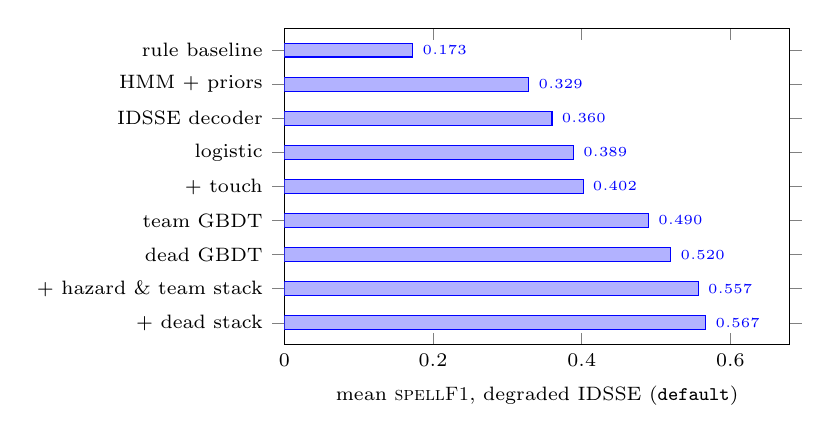
\begin{tikzpicture}
\begin{axis}[
  xbar, width=0.66\columnwidth, height=5.6cm,
  xmin=0, xmax=0.68, xtick={0,0.2,0.4,0.6},
  xlabel={\scriptsize mean \spf{}, degraded IDSSE (\texttt{default})},
  symbolic y coords={final,stack1,deadg,teamg,touch,logit,dec,v1,base},
  ytick=data,
  yticklabels={+ dead stack, + hazard \& team stack, dead GBDT, team GBDT, + touch, logistic, IDSSE decoder, HMM + priors, rule baseline},
  yticklabel style={font=\scriptsize},
  xticklabel style={font=\scriptsize},
  bar width=5pt, enlarge y limits=0.08,
  nodes near coords, nodes near coords style={font=\tiny, /pgf/number format/.cd, fixed, fixed zerofill, precision=3},
  every axis plot/.append style={fill=gray!45, draw=black!70}]
\addplot coordinates {(0.567,final) (0.557,stack1) (0.520,deadg) (0.490,teamg) (0.402,touch) (0.389,logit) (0.360,dec) (0.329,v1) (0.173,base)};
\end{axis}
\end{tikzpicture}
\caption{Ladder of accepted steps. Each bar is held-out \spf{} averaged over the seven degraded IDSSE matches. The hazard-exit step (0.537) is omitted for readability.}
\label{fig:ladder}
\end{figure}

\begin{table}[t]
\caption{Final system by degradation mode (7 matches, held-out).}
\label{tab:final}
\centering
\footnotesize
\begin{tabular}{@{}lrrc@{}}
\toprule
Mode & \spf{} & Gain over previous final & Matches better\\
\midrule
\texttt{default} & 0.567 & $+0.031\pm0.007$ & 7/7\\
\texttt{fused}   & 0.572 & $+0.032\pm0.007$ & 7/7\\
\texttt{harder}  & 0.541 & $+0.028\pm0.008$ & 7/7\\
\texttt{easier}  & 0.596 & $+0.028\pm0.003$ & 7/7\\
\texttt{hidelo}  & 0.546 & $+0.029\pm0.006$ & 7/7\\
\texttt{hidehi}  & 0.598 & $+0.033\pm0.006$ & 7/7\\
\bottomrule
\end{tabular}
\end{table}

\textbf{Tested and dropped.} Table~\ref{tab:rejected} lists what the protocol or the label-free checks rejected. Post-processing of the decoded sequence did nothing: the decoder already enforces durations, so smoothing rules have nothing left to fix. The duration stages are the instructive case. They passed the ladder narrowly, but a control that re-swept $\lambda$ \emph{without} them gained the same, so the gain came from $\lambda$ and the stages were removed.

\begin{table}[t]
\caption{Variants tested and dropped.}
\label{tab:rejected}
\centering
\footnotesize
\begin{tabular}{@{}>{\raggedright\arraybackslash}p{3.3cm}>{\raggedright\arraybackslash}p{4.7cm}@{}}
\toprule
Variant & Result and reason\\
\midrule
Post-processing (midpoint switch, D bridging/crossing, minimum spell) & $|\Delta|\le0.0003$: no gain.\\
Boundary-shift correction learnt on IDSSE & $-0.015\pm0.002$.\\
Dead-ball model fitted on three degradations pooled & $-0.001\pm0.001$.\\
Semi-Markov duration stages & $+0.000\pm0.003$ against a $\lambda$-only control.\\
Pass bridge as input of the logistic team model & Frame AUC 0.92 vs 0.85, but merged adjacent possessions: lower \spf{} in all modes.\\
Control/touch memories in the first-stage team GBDT & Better alone; with the second stages 0.565 vs 0.567.\\
Second stage without hazard input & Worse than with it.\\
Abrupt-touch condition; hazard input \texttt{ball\_dir\_change}; tracked-player counts and team spread in the team GBDT & Failed the label-free feature-shift check on the provided tracking (they depend on ball noise or camera coverage): removed and refitted on IDSSE.\\
Broadcast player tracking & NO-GO at the feasibility gate.\\
\bottomrule
\end{tabular}
\end{table}

\section{Limitations}
\label{sec:limits}

\begin{itemize}
\item \textbf{Domain shift (DFL $\rightarrow$ Metrica).} All parameters come from corrected tracking of another provider and league, degraded synthetically. The degradation matches label-free statistics, but not everything: the rule baseline makes more possessions per minute on degraded IDSSE than on the provided match, and the shares of interpolated ball frames and removed ball jumps differ by more than 20\,\%. The IDSSE scores above are \emph{not} an estimate of the score on the provided match.
\item \textbf{Ball visibility as a dead-ball cue.} To match the provided tracking, the degraded ball is seen on about 30\,\% of dead-ball frames and 80\,\% of live frames, so ``no ball'' is a strong dead-ball cue in training. The \texttt{hidelo}/\texttt{hidehi} modes and the stability check bound this risk but do not remove it.
\item \textbf{Possession convention.} IDSSE labels follow the DFL convention, which may differ from the challenge ground truth on short touches, duels and the exact frame of a change.
\item \textbf{Short possessions.} Before the second stage, recall at IoU 0.5 was 0.04 for possessions under 1\,s, 0.19 for 1--2\,s and 0.93 above 20\,s. The final system still predicts about 310 possessions per match for 437 true ones (\texttt{fused}). It under-segments: fast exchanges are merged.
\item \textbf{Tag recall.} Many restarts have no tag, so dead-ball detection relies on kinematics, which are weakest when the ball is not tracked.
\item \textbf{Ball filter edge cases.} A phantom that stands still for 3\,s or more can beat a sparsely detected real ball, and in a quick multi-ball restart the last frames of the old ball can be removed. A local label-free count found few occurrences in each half, so the filter was not changed.
\item \textbf{Selection noise.} Decoder weights and the set of variants were chosen on the same seven matches (the fitted weights never see the held-out match). Two decisions were taken after a result was known: the fused ball (Section~\ref{sec:assets}) and, in an intermediate step, a hazard weight outside the pre-registered grid. Both passed the same acceptance rule, but the selection is somewhat optimistic. The \texttt{fused} proxy has no stress versions.
\end{itemize}

\textbf{With more time} we would: (i)~give the hazard the team evidence as input (+0.004 in a scratch run, but it needs a third level of nesting); (ii)~target short open-play exchanges directly, e.g.\ with a boundary model trained on IDSSE transitions; (iii)~add labelled data from another provider closer to automatic tracking; (iv)~run our own ball detector on the tactical video to reduce the 41\,\% of frames without a ball; and (v)~rerun the full ladder with the duration control built in.

\section{Reproduction}
\label{sec:repro}

From a clean clone with the data bundle unpacked in \texttt{./data} (and \texttt{MTAH\_DATA\_DIR} unset):
\begin{small}
\begin{verbatim}
python3.12 -m venv .venv
source .venv/bin/activate
pip install -r requirements-modeling.txt
python -m modeling.make_submission \
  --config configs/final.yaml \
  --out outputs/brasileirao.csv
python evaluation/validate_submission.py \
  outputs/brasileirao.csv
\end{verbatim}
\end{small}
The single command runs the preprocessing (with the fused ball), the three first-stage models, the two second stages and the decoder.
\begin{itemize}
\item \textbf{Code:} tag \texttt{submission-v1.1}, config \texttt{configs/final.yaml}. The method is the code-freeze tag \texttt{submission-v1} (commit \texttt{e68d883}); \texttt{v1.1} adds the dependency pins below and documentation only.
\item \textbf{Versions:} Python 3.12; numpy 2.0.2, pandas 2.3.3, pyarrow 21.0.0, scipy 1.13.1, kloppy 3.18.0, PyYAML 6.0.2, scikit-learn 1.5.2, joblib 1.6.0, threadpoolctl 3.8.0 (exact pins in the repository).
\item \textbf{Models:} committed under \texttt{models/} (about 0.5\,MB each); inference refuses another scikit-learn version or feature list.
\item \textbf{Determinism:} CPU, one thread (BLAS and tree models), fixed seeds, explicit \texttt{float64} sums instead of BLAS products, stable sorts. Clean clones on two machines with different CPU generations (Intel Core i7-10750H and i5-1235U) produced the same file, byte for byte (\texttt{docs/reproducibility.md}).
\item \textbf{SHA-256 of \texttt{brasileirao.csv}:}\\ {\footnotesize\texttt{25064d90ff2808ffb325f43d51253a5d}\\\texttt{d58be765d70c2ddee6d608f5fb9f0503}}
\item \textbf{IDSSE is not needed to reproduce the file.} It is needed only to refit the models; that code is in \texttt{modeling/external}, \texttt{modeling/calibration} and \texttt{modeling/scoring}, and \texttt{docs/reproducibility.md} gives the details.
\end{itemize}

\section{How the provided match was used (compliance)}
\label{sec:compliance}

\begin{itemize}
\item \textbf{No human labels and no training on the provided match.} No frame was annotated by hand, and no parameter, weight or threshold was fitted or chosen with labels of this match, including algorithmic pseudo-labels.
\item \textbf{Unlabelled statistics, for the degradation only.} Label-free statistics of the provided tracking (ball visibility, tracked players, speeds, gap lengths) were used only to make the degradation of IDSSE realistic. This is unsupervised use, allowed by RULES.md. The same kind of label-free comparison was used to \emph{remove} features whose distribution on the provided tracking falls outside the IDSSE range; nothing was fitted to it.
\item \textbf{Published constants.} The graded blocks of each half and the kick-off frames are the values published by the organisers (DATA.md, FAQ.md).
\item \textbf{Public window.} Used only for PASS/FAIL correctness checks, never to tune or select anything. Its score is not reported anywhere.
\item \textbf{No frame-specific rules.} No rule or constant is tied to specific frames of the match, other than the published constants.
\item \textbf{Cloud LLMs.} No match data, extract or screenshot was sent to cloud-hosted language models. Coding assistants worked only with synthetic fixtures and the public IDSSE data. Every step that reads the match data was run locally by a team member, and only PASS/FAIL results and statistics of the predicted labels left that machine.
\end{itemize}

\begin{thebibliography}{99}

\bibitem{bassek2025}
M.~Bassek, R.~Rein, H.~Weber, and D.~Memmert, ``An integrated dataset of spatiotemporal and event data in elite soccer,'' \textit{Scientific Data}, vol.~12, art.~195, 2025, doi: 10.1038/s41597-025-04505-y. Licence CC BY 4.0.

\bibitem{idssehf}
PySport, ``idsse-data,'' Hugging Face dataset mirror, revision \texttt{a715a38dfbaf5f58e431727c2b78d174101a703c}. [Online]. Available: \url{https://huggingface.co/datasets/pysport/idsse-data}

\bibitem{mtah2027}
Metrica Sports and Barça Innovation Hub, ``More than a Hack 2027: Frame-level ball possession,'' 2026. [Online]. Available: \url{https://github.com/metrica-sports/more-than-a-hack-2027}

\bibitem{kloppy}
PySport, ``kloppy: Standardizing soccer tracking and event data,'' v3.18.0. [Online]. Available: \url{https://github.com/PySport/kloppy}

\bibitem{rabiner1989}
L.~R. Rabiner, ``A tutorial on hidden Markov models and selected applications in speech recognition,'' \textit{Proc. IEEE}, vol.~77, no.~2, pp.~257--286, 1989.

\bibitem{forney1973}
G.~D. Forney, ``The Viterbi algorithm,'' \textit{Proc. IEEE}, vol.~61, no.~3, pp.~268--278, 1973.

\bibitem{bengio1995}
Y.~Bengio and P.~Frasconi, ``An input output HMM architecture,'' in \textit{Advances in Neural Information Processing Systems 7}, 1995, pp.~427--434.

\bibitem{friedman2001}
J.~H. Friedman, ``Greedy function approximation: A gradient boosting machine,'' \textit{Ann. Statist.}, vol.~29, no.~5, pp.~1189--1232, 2001.

\bibitem{ke2017}
G.~Ke \textit{et al.}, ``LightGBM: A highly efficient gradient boosting decision tree,'' in \textit{Advances in Neural Information Processing Systems 30}, 2017.

\bibitem{pedregosa2011}
F.~Pedregosa \textit{et al.}, ``Scikit-learn: Machine learning in Python,'' \textit{J. Mach. Learn. Res.}, vol.~12, pp.~2825--2830, 2011.

\bibitem{wolpert1992}
D.~H. Wolpert, ``Stacked generalization,'' \textit{Neural Networks}, vol.~5, no.~2, pp.~241--259, 1992.

\bibitem{savitzky1964}
A.~Savitzky and M.~J.~E. Golay, ``Smoothing and differentiation of data by simplified least squares procedures,'' \textit{Anal. Chem.}, vol.~36, no.~8, pp.~1627--1639, 1964.

\end{thebibliography}

\end{document}
